\documentclass[letterpaper, 12pt]{article}

\setlength{\topmargin}{0in}
\setlength{\headheight}{0in}
\setlength{\headsep}{0in}
\setlength{\footskip}{0.5in}
\setlength{\textheight}{\paperheight}
\addtolength{\textheight}{-2in}
\addtolength{\textheight}{-\footskip}

\setlength{\oddsidemargin}{0in}
\setlength{\evensidemargin}{0in}
\setlength{\textwidth}{\paperwidth}
\addtolength{\textwidth}{-2in}

\pagestyle{empty}

\usepackage{amsfonts}
\usepackage{tikz}

\begin{document}

\begin{center}
\bfseries
San Jos\'{e} State University \\
Fall 2015 \\
Math-8: College Algebra \\
Section 03: MW noon--1:15pm \\
Section 05: MW 4:30--5:45pm \\
\bigskip
Quiz \#13 (Solutions)
\end{center}

\bigskip

When a function $f(x)$ has an inverse, we denote the inverse function as
$f^{-1}(x)$. Note that this should note be confused with $\frac{1}{f(x)}$,
which we would denote by $[f(x)]^{-1}$.

\bigskip

Consider the function $f(x)=x^2-4x+3$.

\bigskip

1. Put $f(x)$ in standard form and sketch the graph.

First, complete the square.  Many of you insist on using the $x=-\frac{b}{2a}$
method.  Please learn how to complete the square!

\[f(x) = (x^2-4x+4)+3-4 = (x-2)^2-1\]

So the vertex is $(2, -1)$.  Next, we can factor to find the x-intercepts:

\[f(x)=(x-1)(x-3)\]

and thus the x-intercepts are $(1,0)$ and $(3,0)$.  Please always write these
as points and not just as $x=1,3$.  Finally, for the y-intercept, we set $x=0$:

\[f(0)=(0-1)(0-3)=(-1)(-3)=3\]

So the y-intercept is $(0,3)$.  Putting all of this together, we sketch the
graph as follows:

\bigskip

\begin{center}
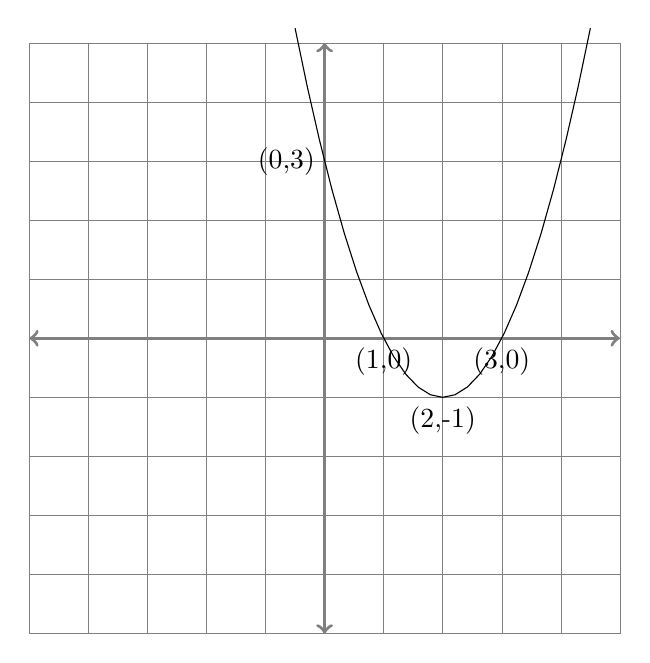
\begin{tikzpicture}[scale=0.75]
\draw [help lines] (-5,-5) grid (5,5);
\draw [help lines, <->, very thick] (-5,0) -- (5,0);
\draw [help lines, <->, very thick] (0,-5) -- (0,5);
\node [below] at (1,0) {(1,0)};
\node [below] at (3,0) {(3,0)};
\node [left] at (0,3) {(0,3)};
\node [below] at (2,-1) {(2,-1)};
\draw [domain=-0.5:4.5] plot (\x, {(\x)^2-4*(\x)+3});
\end{tikzpicture}
\end{center}

\bigskip

2. What is the domain of $f(x)$?

\bigskip

Domain=$(-\infty,\infty)$ (all real numbers).

\bigskip

3. By looking at the graph, does $f(x)$ have an inverse? Why or why not?

\bigskip

No, it fails the horizontal line test.

\bigskip

4. How can the domain of $f(x)$ be adjusted such that it does have an inverse?

\bigskip

We need to adjust the domain so that it can pass the horizontal line test.
Note that the axis of symmetry is $x=2$, i.e., the y values repeat on either
side of the axis.  So, we pick one side.  Correct answers here are
$(-\infty,2]$ or $[2,\infty)$.

\bigskip

5. Using the adjustment you found in (4), find $f^{-1}(x)$.

Setting $f(x)=y$ and solving for $x$ we get:

\begin{eqnarray*}
y &=& (x-2)^2-1 \\
y+1 &=& (x-2)^2 \\
(x-2) &=& \pm\sqrt{y+1} \\
x &=& 2\pm\sqrt{y+1} \\
\end{eqnarray*}

But this is not a function because of the plus/minus.  The sign to select must
match your choice of domain in (4):

\bigskip

\begin{tabular}{|c|c|}
\hline
$(-\infty,2]$ & $x=2-\sqrt{y+1}$ \\
\hline
$[2,\infty)$ & $x=2+\sqrt{y+1}$ \\
\hline
\end{tabular}

\end{document}
